% !TEX root=/home/tavant/these/manuscript/src/manuscript.tex


\section{Presentation of the Hall effect Thruster }
  \label{sec-HET}
  % \addcontentsline{toc}{section}{Presentation of the Hall effect Thruster}

  
  The \ac{HET} is an electrostatic electrical propulsion system accelerating ions by the mean of an imposed voltage difference.
  \Cref{fig-bhtonoff} shows a picture of an \ac{HET} switched on and off.
  We can see the plasma in the annular plasma chamber.


  \begin{figure}[hbt]
    \centering
    \includegraphics[width=\defaultwidth]{PPS-ON_OFF.jpg}
    \caption{Front view of an \acs{HET}, the BHT-1500 from Busek, USA}
    \label{fig-bhtonoff}
  \end{figure}

  We can summarize the composition of an \ac{HET} with four parts\string:
  \begin{enumerate}
    \item The annular chamber.
    \item The injecting anode
    \item The cathode
    \item The magnetic circuit
  \end{enumerate}

  \begin{figure}[hbt]
    \centering
    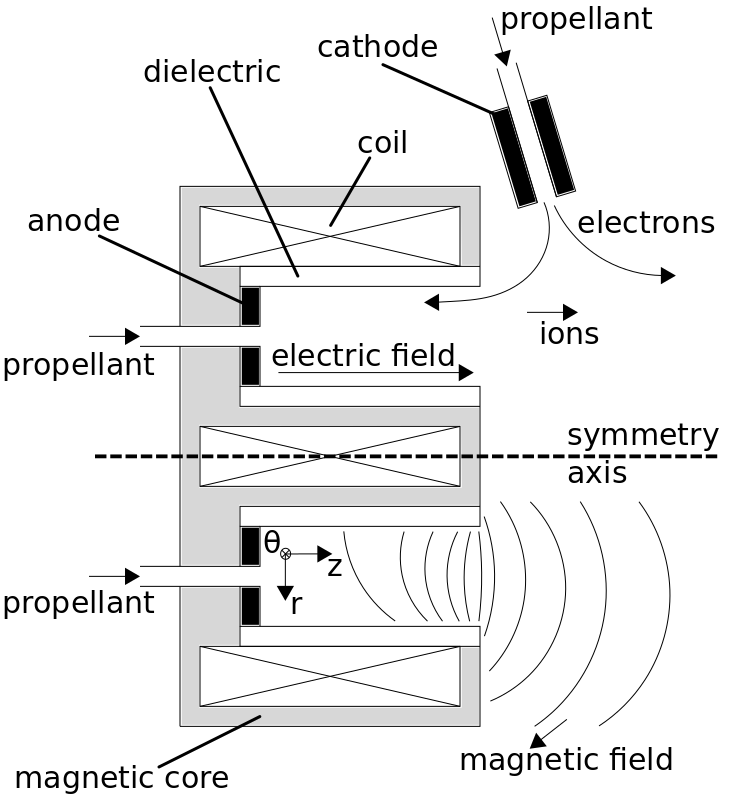
\includegraphics[width=\defaultwidth]{shematic_HET}
    \caption{Schematic cut of an \acs{HET}, illustrating its different parts. }
    \label{fig-shematiccut}
  \end{figure}

  \Cref{fig-shematiccut} presents a schematic cut of the \ac{HET} along its axial and radial direction.

  \paragraph{The chamber} has an annular shape.
  It is closed at the anode side and kept open at the other side.
  The axial length of the chamber is between $1$ and $3\,\centi\meter$; the radial width of the chamber is between $1$ and $2\,\centi\meter$. 
  The walls are usually constituted by a ceramic, as the \ac{BNSiO2}.
  The material needs to be resistant to erosion by ion impact sputtering.
  But changing the material is also known to affect the behavior of the discharge.
  The usually supposed phenomenon for this impact is the secondary electron emission yield that is a function of the material nature.
  For materials used in HET, this yield may be higher than one.


  \paragraph{The anode} is at the bottom of the chamber.
  The anode voltage is imposed to a few hundred volts.
  Usually, the neutral gas is injected through the anode itself, or close to the anode.
  The mass flow rate is of the order of a few mg/s.

  \paragraph{The cathode} is outside of the chamber.
  It is grounded, and injects electrons for two reasons\string:
  \begin{itemize}
    \item most of the electrons ($\sim 90 \%$) are used to neutralize the ion flux, for both allowing the ions to leave the thruster and avoiding charging of the spacecraft,
    \item  the others are attracted by the anode, hence entering the chamber. They enable the plasma discharge to switch and remain on.
  \end{itemize}

  \paragraph{The magnetic circuit} is composed of electromagnets and a magnetic circuit made of different ferromagnetic pieces.
  It creates a constant radial magnetic field in the annular chamber.
  The maximum value of the radial magnetic field is located close to the exit plane of the chamber.
  Its amplitude is on the order of $200$ Gauss ($\sn{2}{-2}$ T).

  \Cref{fig-bshape} illustrates the axial profile of the magnitude of the radial magnetic field.
  \begin{figure}[hbt]
    \centering
    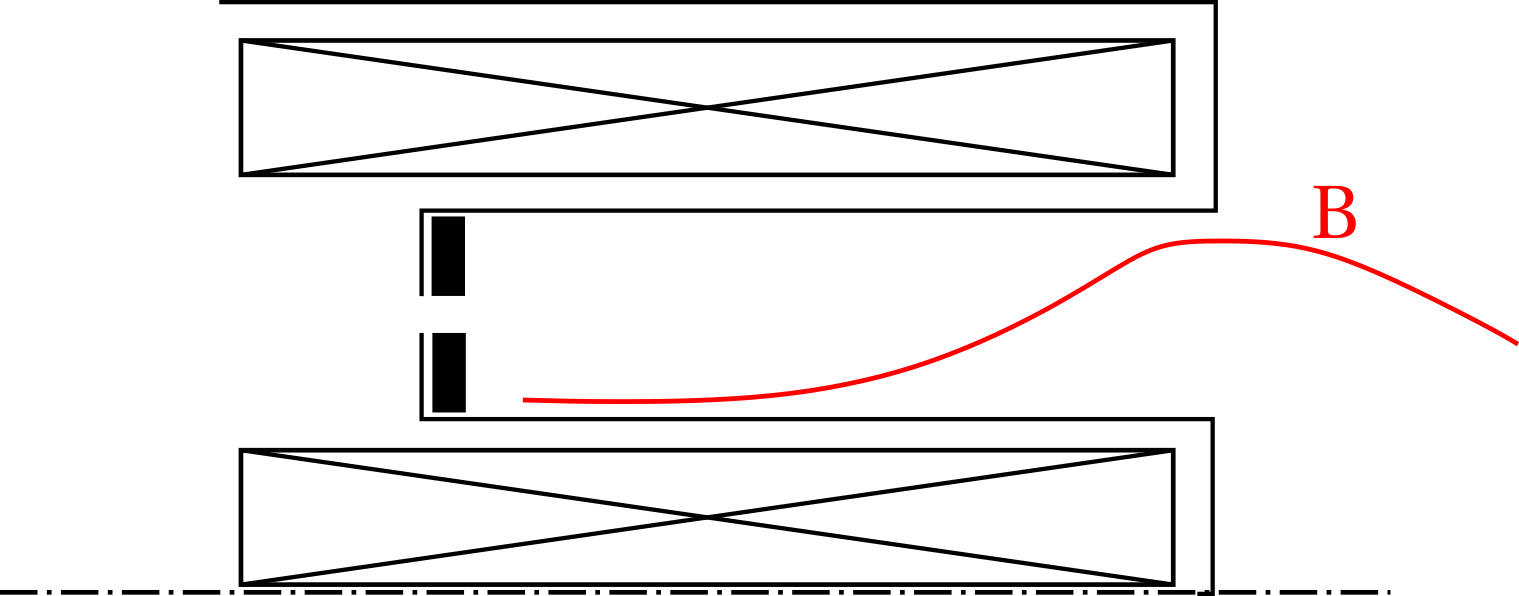
\includegraphics[width=\defaultwidth]{bshape}
    \caption{Usual shape of the axial profile of the radial magnetic field on the centerline of the channel.}
    \label{fig-bshape}
  \end{figure}


\section{HET operating principle}
% \addcontentsline{toc}{subsection}{HET operating principle}


  The operation principle of a \ac{HET} is rather simple.
  The objective is to ionize the propellant and impose an electric field to accelerate the ions.

  \paragraph{Ionization\\}
  The propellant, usually xenon, is ionized by electron-impact.
  The ionization energy needed is $\mathcal{E}_{\rm Xe, iz} = 12.13 \,\volt$, which corresponds to an electron velocity of $2000\,\kilo\meter\per\second$.
  Due to the low pressure (around $\sn{1}{-4}$ Pa), the mean free path of the electrons is larger than the chamber size.
  In consequence, a magnetic field is imposed in order to trap the electrons in a cyclotron motion.
  It increases the residence time of the electrons, thus promotes  ionization.
  In average in a well designed \ac{HET}, 90\% of the propellant is ionized.

  \paragraph{Acceleration\\}
  The potential difference  between the anode and the cathode is used to accelerate the ions outside of the chamber and create the thrust.
  Because the magnetic field slows the electrons down, the plasma resistivity increases in the region where the magnetic field amplitude is large.
  Hence, the axial profile of the magnitude of the axial electric field presents a maximum close to the maximum of the magnetic field.
  While the typical voltage difference is $U_d=300\,\volt$, the maximum electric field can be of the order of $30\,\kilo\volt\per\meter$ \citep{gawron2008}.

  \paragraph{Ionization and Acceleration regions overlap\\}
  \Cref{fig-zones} shows an illustration of the usual axial profiles of the ionization and the electric and magnetic fields.
  As the magnetic field governs both the ionization and the acceleration regions, it can be challenging to obtain a clear separation between the two regions.
  However, if ionization happens in the acceleration region, the newly created ions will not be accelerated at their maximum velocity, hence resulting in a loss compared to the maximum theoretical thrust.
  The theoretical maximum speed is, by conservation of the total energy of the ion
  \begin{equation} \label{eq-vmaxtheo}
    v_{\rm ex, max} = \sqrt{ \frac{2 e V}{m_i} } \sim 31 \,\kilo\meter\per\second
  \end{equation}
  with $m_i = 131 \,\atomicmass$ for xenon and $V=300\,\volt$.


  \begin{figure}[hbt]
    \centering
    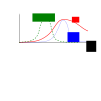
\includegraphics[width=\defaultwidth]{zones}
    \caption{Illustration of the usual axial profiles of the ionization and acceleration amplitude compared to the magnetic field.}
    \label{fig-zones}
  \end{figure}

  The thruster efficiency, in the usual configuration, is governed by its magnetic field topology.
  Hence, it can be tough to find the best topology that will optimize the ionization and the location of the ionization and acceleration regions.
  Some concepts of double stage \ac{HET} have been proposed to decouple the two phenomena to control them independently and are still under study \citep{dubois2018}.
  
  % However, the preliminary results are not as satisfactory as expected. 
  % \inlinenote{Add referecne here}
  % Moreover, the double-stage system needs more parts and power sources, resulting in a more complicated system.

  
  \section{Instabilities present in the \acs{HET} }
  \label{sec-physics}
  % \addcontentsline{toc}{subsection}{Instabilities present in the \acs{HET}}

  The \ac{HET}s are subject to numerous plasma oscillations, over a broad range of frequencies \citep{boeuf2017,choueiri2001}.
  The most important ones are\string:
  \begin{enumerate}
    \item Low frequency (10-20\,\kilo\hertz) ionization oscillations, usually referred to as breathing mode,
    \item Azimuthal low frequency rotating spokes, also in the \kilo\hertz{} range,
    \item Axial ion transit time oscillations, of the order of 100-500 \kilo\hertz,
    \item Azimuthal fast oscillations, of frequency of the order of the ion plasma frequency.
  \end{enumerate} 

  \paragraph{1. Breathing mode\\}
  The breathing mode is relatively understood \citep{boeuf1998,barral2009,hara2014}.
  Indeed, a simple predator-prey model of two equations is enough to obtain qualitatively the observed behavior.
  It is related to the idea that when the ionization is important, the neutral atom density decreases, reducing the ionization.
  Hence, the plasma density decreases, allowing the neutral density to rise again until the ionization grows up again.
  

  \paragraph{2. Rotating spokes\\}
  Experimental measurements with segmented anode \citep{ellison2012,mcdonald2011} seem to indicate that rotating spokes are present in the anode region.
  Their physical origins are less understood, as they were first attributed to ionization \citep{janes1966} but were later related to Simon-Hoh instability, and they were observed in \ac{PIC} simulations even with neglecting ionization \citep{carlsson2018}.
  However, in recent experiments, the presence of spokes did not seem to affect the \ac{HET} performances \citep{boeuf2017}.

  \paragraph{3. Transit time instability\\}
  Transit time instability has been predicted and observed in analytical and numerical models, respectively \citep{barral2005,boeuf2018}.
  Experimental studies of these instabilities are rather scarce, and it is only recently that time-resolved Laser-Induced Fluorescence measurements of the local ion velocity distribution function have confirmed the presence of this instability in a Hall thruster \citep{vaudolon2015}.
  This oscillation could reduce the performance of the thruster by increasing the overlap between the acceleration and ionization regions \citep{boeuf2018}.

  \paragraph{4. High-frequency azimuthal oscillations\\}
  These oscillations were first observed in \ac{PIC} simulations \citep{adam2004,ducrocq2006,adam2008a,heron2013} before being witnessed by electron Thomson scattering \citep{tsikata2009a,tsikata2009,tsikata2013}.
  They are essential, as they enhance the electron transport in the axial direction \citep{adam2004,lafleur2016a}.
  They are further described in the next section.
